We now review the protocol presented in \cite{giordani2020} which utilises quantum walk dynamics in order to generate higher dimensional entanglement. 

In this section we use following notation:
\begin{itemize}
    \item $\ket{u}^{(i)}$ is a state belonging to the subspace $\mathcal{H}^{(i)} = \mathcal{H}^{(i)}_C \otimes \mathcal{H}^{(i)}_W, i\in\{1,2\}$.
    \item $\ket{u}_J$ is a state belonging to the subspace $\mathcal{H}_J = \mathcal{H}^{(1)}_J \otimes \mathcal{H}^{(2)}_J, J\in\{C,W\}$.
    \item  $\ket{u}^{(i)}_J$ is a state belonging to the subspace $\mathcal{H}^{(i)}_J$.
\end{itemize}

In this mathematical framework the overall Hilbert space of the quantum system is comprised of two quantum walk subspaces,
\begin{align}
    \mathcal{H} &= \mathcal{H}^{(1)} \otimes \mathcal{H}^{(2)}\\
                &= \mathcal{H}^{(1)}_C \otimes \mathcal{H}^{(1)}_W \otimes \mathcal{H}^{(2)}_C \otimes \mathcal{H}^{(2)}_W.
\end{align}

The basic premise of this protocol is this:
\begin{enumerate}
    \item Entangle the two coin spaces of the walkers $\mathcal{H}^{(i)}_C$. (Fig \ref{fig:preparation}.)
    \item Proceed with the random walk.
    \item Use a projection $\mathcal{P}_\gamma = \ket{\gamma}\bra{\gamma}, \ket{\gamma}\in\mathcal{H}^{(1)}_C$ to then transfer the entanglement so that it solely exists in the subspace $\mathcal{H}^{(1)}_W \otimes \mathcal{H}^{(2)}_C \otimes \mathcal{H}^{(2)}_W$.
    \item In similar fashion, find a projection $\mathcal{P}_\delta = \ket{\delta}\bra{\delta}, \ket{\delta}\in\mathcal{H}^{(2)}_C$ to transfer the entanglement to exist between the two walker subspaces, $\mathcal{H}^{(i)}_W$, only. 
    \item Accumulate entanglement in the walker subspaces by once more entangling the two coin spaces and repeating the protocol.
\end{enumerate}

\begin{figure}
    \centering
    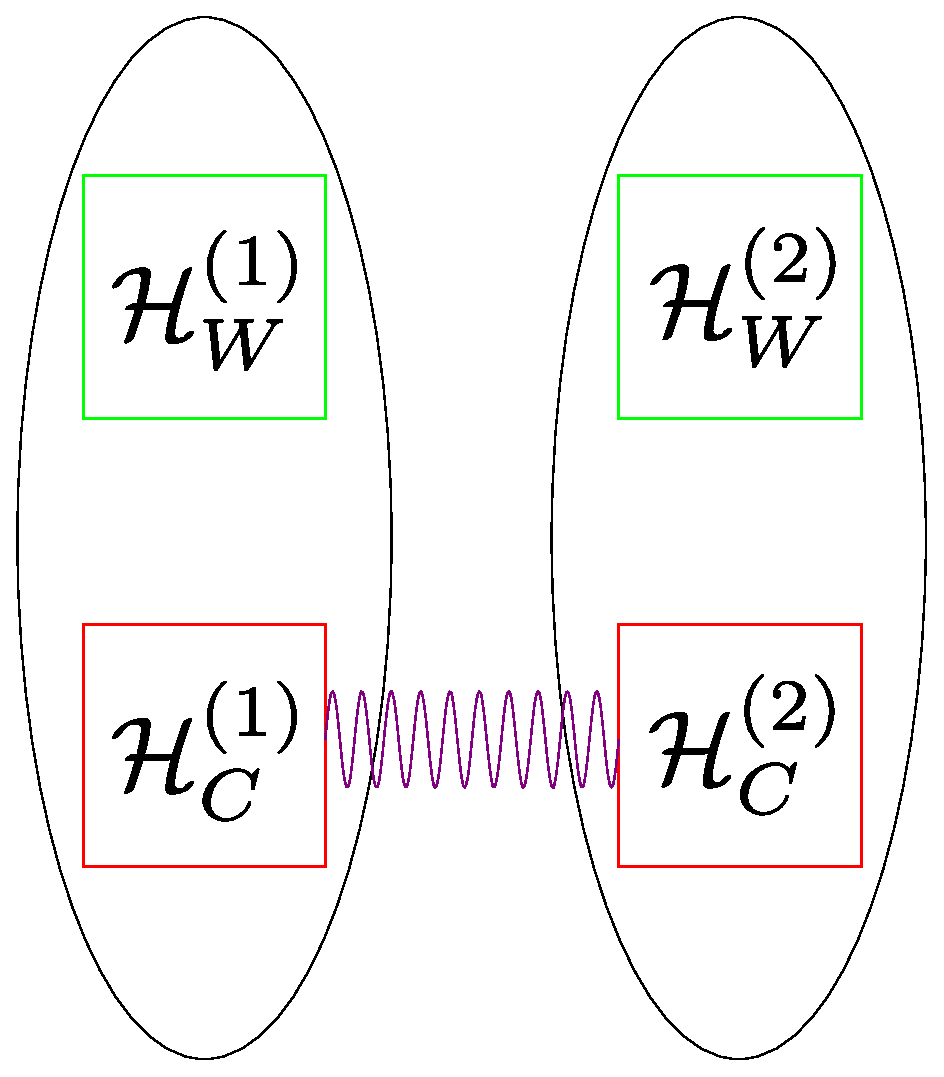
\includegraphics[scale = .25]{preparation}
    \caption{The initial prepared state has entanglement solely between the two coin subspaces. Figure is an edited version from FIG 3 from \cite{giordani2020}.}
    \label{fig:preparation}
\end{figure}

In this way, we are able to generate arbitrary amounts of high dimensional entanglement. 
As is the case with many quantum walk based protocols, particular attention must be paid to the choice of coin used for the quantum walk, as it will have a large impact on the success of the protocol.
In the presentation of the protocol in \cite{giordani2020}, the shift operator $\tilde{S}$ (the operator with no left moving part) is used, and as such we will too present this overview using the same shift operator. It should be noted however, that the choice of shift operator, $S$ or $\tilde{S}$, has no real impact upon the workings of this protocol.

\subsection{Transfer using identity coin operator}
We first use the example of a quantum walk with coin $I$, the identity. We prepare a state $\ket{\psi(0)}$ with the coin states entangled and walkers at the origin
\begin{equation}
    \ket{\psi(0)} = \underbrace{\frac{1}{\sqrt{2}}\Big [\ket{\uparrow}^{(1)}_C\ket{\uparrow}^{(2)}_C + \ket{\downarrow}^{(1)}_C\ket{\downarrow}^{(2)}_C \Big]}_{\text{Bell State}}\otimes \ket{0}^{(1)}_W\ket{0}^{(2)}_W.
\end{equation}
Following this we apply our coin, $I$, and then use our shift operator $S$ to advance the quantum walk. Explicitly (dropping the indices and combining some of our kets together) we obtain
\begin{equation}
    \ket{\psi(1)} = \tilde{S}I\ket{\psi} = \frac{1}{\sqrt{2}}\Big [\ket{\uparrow,\uparrow}\ket{0,0} + \ket{\downarrow,\downarrow}\ket{1,1}\Big].
\end{equation}
We then project the part of $\ket{\psi(1)}$ residing in the $\mathcal{H}^{(1)}_C$ subspace onto the vector $\ket{\gamma}$, using the projective operator $\mathcal{P}_\gamma = \ket{\gamma}\bra{\gamma} \in \mathcal{H}^{(1)}_C$. Choose $\ket{\gamma} = \frac{1}{\sqrt{2}} \big [\ket{\uparrow} + \ket{\downarrow} \big]$ which then gives us
\begin{equation}
    \mathcal{P}_\gamma \ket{\psi(1)} = \frac{1}{2}\Big [\ket{\gamma}\otimes \big (\ket{\uparrow, 0, 0} + \ket{\downarrow, 1, 1}\big )\Big ].
\end{equation}
Similarly, we project the other walker subspace to $\ket{\delta}$ which we can in this instance take to be the same state as $\ket{\gamma} = \frac{1}{\sqrt{2}} \big [\ket{\uparrow} + \ket{\downarrow} \big]$,
\begin{equation}
    \mathcal{P}_\delta \mathcal{P}_\gamma \ket{\psi(1)} = \frac{1}{2\sqrt{2}}\Big [\ket{\gamma}\otimes \ket{\delta} \otimes \frac{1}{\sqrt{2}}\Big (\ket{0, 0} + \ket{1, 1}\Big )\Big ].
\end{equation}
Renormalising we see that we have the state
\begin{equation}
    \ket{\gamma}^{(1)}_C \otimes \ket{\delta}^{(2)}_C \otimes \underbrace{\frac{1}{\sqrt{2}}\Big [\ket{0, 0} + \ket{1, 1}\Big ]_W}_{\text{Bell State}},
\end{equation}
which has a Bell State in the $\mathcal{H}_W$ subspace, and the states in $\mathcal{H}_C$ are separable. Therefore we have transferred the entanglement that originally resided in the coin subspace to the walker one.

\subsection{Accumulation}
Of course the real interest in this protocol, as previously stated, is the ability to accumulate the entanglement transferred from the lower dimensional coin subspace to the higher dimensional walker one. We now demonstrate how we can do this, again using $I$ as our coin. We start with the final state obtained in the previous section (equation (22)) and re-entangle the coin subspaces, redefining the resulting state as our $\ket{\psi(0)}$,
\begin{align}
    \ket{\gamma}^{(1)}_C \otimes \ket{\delta}^{(2)}_C &\otimes \frac{1}{\sqrt{2}}\Big [\ket{0, 0} + \ket{1, 1}\Big ]_W\\
    \overset{\text{Entangle }\mathcal{H}_C}{\longrightarrow} \frac{1}{\sqrt{2}} \Big [\ket{\uparrow, \uparrow} + \ket{\downarrow, \downarrow}\Big ]_C &\otimes \frac{1}{\sqrt{2}}\Big [\ket{0, 0} + \ket{1, 1}\Big ]_W\\
    &=\ket{\psi(0)}.
\end{align}
We then proceed with the walk, however taking two steps instead of one this time,
\begin{align}
    \ket{\psi(2)} &= (\tilde{S}I)^2\ket{\psi(0)}\\
    &= \frac{1}{2}\Big[\ket{\uparrow,\uparrow}\big (\ket{0,0}+\ket{1,1}\big ) + \ket{\downarrow,\downarrow}\big (\ket{2,2} + \ket{3,3}\big )\Big ].
\end{align}
We use the same projectors in the two coin subspaces, $\mathcal{P}_\gamma \in \mathcal{H}^{(1)}_C,  \mathcal{P}_\delta \in \mathcal{H}^{(2)}_C$, and after renormalisation have the final state
\begin{equation}
    \ket{\gamma}\otimes\ket{\delta}\otimes\frac{1}{2}\Big[\ket{0,0} + \ket{1,1} + \ket{2,2} + \ket{3,3}\Big ].
\end{equation}

In this way we have now accumulated two ebits in the walker subspace, and can continue to repeat this process to accumulate arbitrarily large amounts of entanglement into our walker subspace, noting that each $n^{th}$ iteration requires an additional $2^{n-1}$ steps in our quantum walk.

\subsection{Drawbacks}
In the example given above, which is the example given in \cite{giordani2020}, we have demonstrated that this protocol can transfer all of the entanglement to our qudits.
However we are left with a crucial problem in that the example does not in fact use quantum walk dynamics to transfer the entanglement, seeing as there effectively is no coin driving the walk.
In analysing the protocol with the Hadamard coin, I found that only one ebit of entanglement could be transferred efficiently and subsequent repetitions of the protocol to store further amounts of entanglement could not be done optimally.
Simulations of the protocol found that at most around 1.6 ebits of entanglement can be stored with a Hadamard QW, as shown in Figure X.
Furthermore, the projective measurements employed as part of the protocol mean that it is not unitary and is non trivial to reverse in order to retrieve the entanglement out from the entangled qudits.
The experimental implementation suggested in the paper also required the use of post selection, where undesirable states were discarded and the protocol run again.
All this in combination results in a protocol which is rather inefficient in achieving its aims.
However, the example clearly shows that it is possible to efficiently transfer entanglement to qudits, but highlights that a different quantum computational model should perhaps be employed.
In the \S{4}, an alternative protocol in the ancilla-based quantum computing model is proposed which solves most of the inefficiencies present in this QW based proposal.